% Welcome! This is the unofficial University of Udine beamer template.

% See README.md for more informations about this template.

% This style has been developed following the "Manuale di Stile"
% (Style Manual) of the University of Udine. You can find the
% manual here: https://www.uniud.it/it/ateneo-uniud/ateneo-uniud/identita-visiva/manuali-immagine-stile/manuale-stile

% Note: for some reason, the RGB values specified in the manual
% do NOT render correctly in Beamer, so they have been redefined
% for this document using the high level chromo-optic deep neural 
% quantistic technology offered by Microsoft Paint's color picker.

% We defined four theme colors: UniBrown, UniBlue, UniGold
% and UniOrange. For example, to write some uniud-brownish
% text, just use: \textcolor{UniBrown}{Hello!}

% Note that [usenames,dvipsnames] is MANDATORY due to compatibility
% issues between tikz and xcolor packages.

\documentclass[usenames,dvipsnames,xcolor=table]{beamer}
\usepackage[utf8]{inputenc}
\usepackage{tikz}
\usetikzlibrary{calc, shapes.misc}
\usepackage{verbatim}
\usetheme{uniud}

%%% Bibliography
\usepackage[style=authoryear,backend=biber]{biblatex}
\addbibresource{bibliography.bib}

% Author names in publication list are consistent 
% i.e. name1 surname1, name2 surname2
% See https://tex.stackexchange.com/questions/106914/biblatex-does-not-reverse-the-first-and-last-names-of-the-second-author
\DeclareNameAlias{author}{given-family}

%%% Suppress biblatex annoying warning
\usepackage{silence}
\WarningFilter{biblatex}{Patching footnotes failed}

%%% Some useful commands
% pdf-friendly newline in links
\newcommand{\pdfnewline}{\texorpdfstring{\newline}{ }} 
% Fill the vertical space in a slide (to put text at the bottom)
\newcommand{\framefill}{\vskip0pt plus 1filll}


\title[Steel defect detection]{An effective approach to steel defect detection}
\date[\today]{\today}
\author[Antonio Terpin e Claudio Verardo]{
  Antonio Terpin e Claudio Verardo
}
\institute{Scuola Superiore, University of Udine}

\begin{document}

\begin{frame}
\titlepage
\end{frame}

\begin{frame}{Outline}
\tableofcontents
\end{frame}

\section{Introduction}
    \par{
        A fundamental aim in any industry is to design highly efficient and effective quality control processes. Therefore, the research area focusing on automatic defect detection systems has become even more fecund in the last decades. 
    }
    \par{
        There is a large variety of previous work on defect detection on steel surfaces \cite{ieee:4777721, ieee:7030439, ieee:8623728, ieee:1334512, ieee:6738559}. Many ideas \cite{ieee:4777721, ieee:7030439, ieee:8623728} bank on the uniformity of the background surface, while other solutions use deep learning architectures \cite{ieee:1334512, ieee:6738559}, which provide an attempt to a robust defect segmentation. More refined approaches rely on wavelets to detect abrupt changes on the surfaces \cite{ieee:993164, ieee:6703333, ieee:7155940, sciencedirect:NGAN2011442}. 
    }
    \par{
        The core of the architecture proposed in this paper is based on wavelet analysis and on deep learning, due to two main reasons. Firstly, multi-resolution analysis (MRA) based on wavelets was proven effective in facing localization in both spatial and frequency domains. \cite{Vetterli:1995:WSC:201007, Daubechies:1992:TLW:130655, intechopen:bernardini}. This because of wavelet transform mathematical properties, compared to Fourier's transform.
    }
    \par{
        Secondly, in the last years deep learning \cite{Goodfellow:2016:DL:3086952, Rojas:1996:NNS:235222} has outperformed any human-designed classificator. Indeed, computer vision and image processing are increasing in popularity in many fields, from autonomous driving vehicles to retail security. Hence, since the rise of deep learning applications \cite{researchgate:deeplearning} there has been an appreciable improvement in the effectiveness of defect detection based on visual systems and a lot of work has been done.
    }
    \par{
        Three main computer vision tasks can be outlined: classification, object localization and object detection.
    }
    \par{
        The classification task faces the supervised learning problem of identifying to which of a set of categories a given object belongs to. In computer vision this means assigning one of the available labels to an image. This is the simplest of the three tasks, and recognizing the category of the principal object in a picture is the standard application of Convolutional Neural Network (CNN). Examples of usage are identifying handwritten characters \cite{nips:NIPS1989_293, ieee:6248110}, house numbers \cite{ieee:6460867} and traffic signs \cite{ieee:6248110}.

    }
    \par{
        The main reason why CNNs have become so popular since LeCun originally introduced them \cite{nips:NIPS1989_293, ieee:726791, LeCun:1999:ORG:646469.691875, researchgate:deeplearning} is that they represent a black box from raw pixels to categories labels, therefore they overcome the difficulties intrinsic in designing tailored features extractors. Morover, they are also more likely to be shift and scale invariant \cite{LeCun:1999:ORG:646469.691875}, and they have been proven to have enviable classification accuracies.
    }
    \par{
        A classification task in defect detection field is accounted when objects, e.g. steel surfaces, need to be binarily classified as defective or flawless. In monitoring applications, classifying pictures as a whole would be expensive, since local screening hardware would be needed. Patently, a global visual system is far more appetible. 
    }
    \par{
        Moreover, a local analysis may miss some global features of a particular defect; this is the case of burst defects, such as zipper cracks \cite{defects:mainlinemetals}.
    }
    \par{
        Object localization sights to find a given number of items in a given context, predicting both their position and their class. Object detection removes the constraint on the number of items, allowing either zero or any finite number of objects, not fixed \emph{a priori}. In computer vision, in particular in 2D images, the position is described by a bounding box.
    }
    \par{
        CNNs have been used along with sliding window and multiscale approaches for object detection \cite{ieee:7410526, ieee:7532516, arXiv:1312.6229S}, and there is a lot of work aiming to improve performances and bounding boxes accuracies, either by designing different neural network architectures \cite{ieee:7410526} or by tailoring existing one \cite{ieee:726791}.
    }
    \par{
        In this paper, a further refined system is presented, since the purpose of the defect detection algorithm is not only to globally mark a steel surface as flawless or defective from its picture, but to highlight flawed regions within the image and to label them as belonging to a particular defect class.
    }
    \par{
        Pixel-wide classification is known in literature as image segmentation, and there are three main families of tecniques: hysteretic thresholding, edge-based and region-based \cite{ieee:7684170}. Thresholding exploits a previously known function defined over the pixels space and classifies pixels through comparison with some discrete values (thresholds) \cite{ieee:4310039}, but it is tipically used within other tecniques rather then alone. Region-based approaches use either graph algorithms \cite{ieee:6205760, ieee:868688} or watersheds analogies \cite{ieee:87344}. Edge-based tecniques, instead, use an edge detection filter \cite{Klette:2014:CCV:2584519, googlescholar:kovesiphase, researchgate:phase}, along with denoising and thresholding considerations, to solve the boundary detection problem. Remark that, although similar, boundary detection aims to describe changes in pixel ownerwhip from one object or surface to another, whereas an edge is an abrupt change, which can be a sub-domain of a border. There are also more advanced boundary-related tecniques \cite{springer:Kass1988} which rely on energy minimization and are embedded on region-based approaches. Indeed, all these tecniques can be mixed both together and with learning algorithms, either unsupervised \cite{ieee:7684170} or supervised \cite{ieee:1273918}.
    }
    \par{
        The approach here described merges the more effective and efficient ideas of previously described work, balancing the drawbacks of different tecniques. Since segmentation is needed, an edge-based contour detector is presented, to reach high speed segmentation. Wavelet are used along with image preprocessing and alpha-shape \cite{springer:10.1007/11907350_46} to identify proposals, i.e. regions of interest for the classificator, which may contain a defective area. To overcome the bias introduced from hand-crafting the edge-detection filter, the hyperparameters of the algorithm are tuned with Bayesian Optimization \cite{arXiv:2018arXiv180702811F, arXiv:2012arXiv1206.2944S, rasmussen:williams:2006}.
        A multi-column CNN (MC-CNN) \cite{ieee:6248110} is then used to combine the segmentation information with a well-known classificator architecture, exploiting both local information and global information. The preliminary implementation of the proposed architecture has shown good performances on the \emph{Severstal: Steel Defect Detection} Kaggle competition dataset \cite{kaggle:severstal}.
    }
\section{Defect detection}

\framepic{graphics/architecture/defect-detection}{
    \framefill
    \textcolor{white}{An effective approach to steel defect detection}
    \vskip 0.5cm
}

\begin{frame}{Defect detection on steel surfaces}
    \onslide <1-> {
        \includegraphics[width=\textwidth]{graphics/architecture/architecture-input}
    }
    \onslide <2-> {
        \includegraphics[width=\textwidth]{graphics/architecture/architecture-output}
    }
\end{frame}

\subsection{Data Analysis}
    \framepic{graphics/defects/dataanalysis}{
        \framefill
        \textcolor{black}{Data Analysis}
        \vskip 0.5cm
    }

    \begin{frame}
        \frametitle{Data Analysis}
        \framesubtitle{Data augmentation}
        TODO fix statistics image
    \end{frame}

    \begin{frame}
        \frametitle{Data Analysis}
        \framesubtitle{Defect analysis}
        \includegraphics[width=\textwidth]{graphics/defects/class1surface}\\
        \includegraphics[width=\textwidth]{graphics/defects/class1surface-highlighted}\\
        \includegraphics[width=\textwidth]{graphics/defects/class1shape}
    \end{frame}

    \begin{frame}
        \frametitle{Data Analysis}
        \framesubtitle{Defect analysis}
        \includegraphics[width=\textwidth]{graphics/defects/class2surface}\\
        \includegraphics[width=\textwidth]{graphics/defects/class2surface-highlighted}\\
        \includegraphics[width=\textwidth]{graphics/defects/class2shape}
    \end{frame}

    \begin{frame}
        \frametitle{Data Analysis}
        \framesubtitle{Defect analysis}
        \includegraphics[width=\textwidth]{graphics/defects/class3surface}\\
        \includegraphics[width=\textwidth]{graphics/defects/class3surface-highlighted}\\
        \includegraphics[width=\textwidth]{graphics/defects/class3shape}
    \end{frame}

    \begin{frame}
        \frametitle{Data Analysis}
        \framesubtitle{Defect analysis}
        \includegraphics[width=\textwidth]{graphics/defects/class4surface}\\
        \includegraphics[width=\textwidth]{graphics/defects/class4surface-highlighted}\\
        \includegraphics[width=\textwidth]{graphics/defects/class4shape}
    \end{frame}
\subsection{Proposed architecture}

\framepic{graphics/architecture/architecture}{
    \framefill
    \textcolor{white}{Proposed architecture}
    \vskip 0.5cm
}

\begin{frame}[fragile]{Proposed architecture}
    \vskip -0.5cm
    \begin{block}{Region-based CNN (R-CNN)}
        \begin{itemize}
            \item Region proposals
            \item Classification
        \end{itemize}
    \end{block}
    \vskip 0.25cm
    \centering
    \begin{tikzpicture}
        % Input
        \node[rectangle, draw, minimum width=2cm, minimum height=2cm, anchor=west] at (-2,0) {Image};

        % \onslide <2-> {
            \draw[->] (0.5,0) -- (1.5,0);

            % Region proposals
            \node at (2.5,1.5) {Region proposals};
            \foreach \i in {0,...,7}
                \node[rectangle, draw, minimum width=1cm, minimum height=1cm, anchor=north west, fill=white] at (2 +\i*0.2,1-\i*0.2) {};
        % }

        % \onslide <3-> {
            \draw[->] (4.5,0) -- (5.5,0);

            % Classification
            \node at (5.5,1.5) {Class};
            \draw[->, color=UniBlue] (6.2, .8) -- (5.7, 1.25);
            \draw[color=UniBlue] (6.35,-.25) ellipse (0.25cm and 1.1cm);

            \node at (8.2,2) {Encoded};
            \node at (8.3,1.5) {Pixels};
            \draw[->, color=UniOrange] (7, .95) -- (7.5, 1.55);
            \draw[color=UniOrange] (7.6,.6) ellipse (1.1cm and 0.35cm);

            \node [matrix, anchor=north west, draw] at (6,1)
            {
                % \node {Class}; & \node {EncodedPixels};\\
                \node {$1$}; & \node {``12 13 \ldots''};\\
                \node {$2$}; & \node {``6 35 \ldots''};\\
                \node {$3$}; & \node {``''};\\
                \node {$4$}; & \node {``192 78 \ldots''};\\
            };
        % }
    \end{tikzpicture}
\end{frame}

\subsubsection{Region proposals}
\begin{frame}{Region proposals}
    TODO include original image
    TODO include edged image
    TODO include alpha-shape
    TODO include bounding boxes
\end{frame}

\begin{frame}
    \frametitle{Edge-based image segmentation}
    \framesubtitle{Edge Detection}
    \includegraphics[width=\textwidth]{graphics/computervision/edge-odd}
    \includegraphics[width=\textwidth]{graphics/computervision/edge-odd-plot}
    \begin{exampleblock}{Odd transition}
        Given a function defined on a $2D$ domain, a local odd transition is likely to describe border edge.
    \end{exampleblock}
\end{frame}

\begin{frame}
    \frametitle{Edge-based image segmentation}
    \framesubtitle{Edge Detection}
    \includegraphics[width=\textwidth]{graphics/computervision/edge-even}
    \includegraphics[width=\textwidth]{graphics/computervision/edge-even-plot}
    \begin{exampleblock}{Even transition}
        Given a function defined on a $2D$ domain, a local even transition is likely to describe a line.
    \end{exampleblock}
\end{frame}
    
\begin{frame}
    \frametitle{Edge-based image segmentation}
    \framesubtitle{Phase Congruency}
    \begin{block}{Phase-congruency model}
        Given $v_1, v_2, \ldots, v_n \in \mathcal{V}$, their phase congruency is defined as:
        \begin{equation}
            \mathcal{P} = \frac{\lvert \sum_{i} v_i \rvert}{\sum_{i} \lvert v_i \rvert}
        \end{equation}
    \end{block}
    \centering
    \includegraphics[width=0.6\textwidth]{graphics/computervision/phasecongruency}
\end{frame}

\begin{frame}
	\frametitle{Edge-based image segmentation}
	\framesubtitle{Kovesi Algorithm}
	Algorithm
\end{frame}

\begin{frame}
	\frametitle{Edge-based image segmentation}
	\framesubtitle{Hysteretic Edge Follower}
	\begin{block}{Algorithm}
	  	Let $\mathcal{I}$ be the image, $\mathcal{Q} = \left\{q \in \mathcal{I} \colon \hat{\mathcal{P}}(q) > T_{high}\right\}$, $\Omega(q)$ the set of  pixels adjacent to $q$ and $\mathcal{E} = \empty$ the set of edge pixels.
		Then, the hysteretic edge follower calculates edge pixels as:
		\begin{enumerate}
			\item $q_i \in \mathcal{Q};\; \mathcal{Q} = \mathcal{Q} \setminus \{q_i\};\;\mathcal{E} = \mathcal{E} \cup \{q_i\}$
			\item $\forall q_j \in \Omega(q_i)$ if $\hat{\mathcal{P}}(q_j) > T_{low}$ then $\mathcal{E} = \mathcal{E} \cup \{q_j\}$ and repeat $(2)$ with $q_i = q_j$
			\item if $\mathcal{Q} \neq \emptyset$ then repeat $(1)$
		\end{enumerate}
	\end{block}
\end{frame}

\begin{frame}
	\frametitle{Edge-based image segmentation}
	\framesubtitle{Hysteretic Edge Follower}
	\only<1-4> {
		\includegraphics[width=\textwidth]{graphics/architecture/detector-ex}
	}
	\only<2-4> {
		\includegraphics[width=\textwidth]{graphics/architecture/detector-ex-hysteresis-30-50}
	}
	\only<3-4> {
		\includegraphics[width=\textwidth]{graphics/architecture/detector-ex-hysteresis-60-100}
	}
	\only<4-4> {
		\includegraphics[width=\textwidth]{graphics/architecture/detector-ex-hysteresis-90-150}
	}
\end{frame}

\begin{frame}
    \frametitle{Edge-based image segmentation}
    \framesubtitle{$\alpha$-Shape}
    \begin{columns}[onlytextwidth]
        \column{0.5\textwidth}
            \onslide <1-> {
                \includegraphics[width=\textwidth]{graphics/computervision/detector-points}
            }
        \column{0.5\textwidth}
            \onslide <2-> {
                \includegraphics[width=\textwidth]{graphics/computervision/detector-a-shape-better-radius}
            }
    \end{columns}
%    \onslide <3-> {
%        \begin{theorem}[Topologically correct image segmentation]
%            Under certain conditions on the parameters of the alpha-shape, the boundary reconstruction is topologically equivalent to the boundary of the original region.
%        \end{theorem}
%    }
\end{frame}

\begin{frame}
	\frametitle{Edge-based image segmentation}
	\framesubtitle{$\alpha$-Shape}
	\only<1-3> {
			\includegraphics[width=\textwidth]{graphics/architecture/detector-ex}
	}
	\only<2-3> {
			\includegraphics[width=\textwidth]{graphics/architecture/detector-ex-segmentated}
	}
	\only<3-3> {
			\includegraphics[width=\textwidth]{graphics/architecture/detector-ex-bounding-box}
	}
\end{frame}

\begin{frame}
    \frametitle{Region proposals}
    \framesubtitle{Optimization}
    \onslide <1-> {
        \begin{alertblock}{Kovesi algorithm tuning}
            Parameters: $N$, $U$, $\lambda$ and $s$.
        \end{alertblock}
    }
    \onslide <2-> {
        \begin{alertblock}{Hysteretic edge follower tuning}
        	Parameters: $T_{low}$ and $T_{high}$.
        \end{alertblock}
    }
    \onslide <3-> {
        \begin{alertblock}{Alpha shape tuning}
        	Parameters: $\alpha$, $T_{hole}$ and $T_{regions}$.
        \end{alertblock}
    }
    \onslide <3-> {
        \begin{exampleblock}{Parameters tuning - solution}
            An empirical approach is proposed: \textbf{Bayesian optimization} is used to tune the hyper parameters of the algorithm.
        \end{exampleblock}
    }
\end{frame}

\begin{frame}
	\frametitle{Region proposals}
	\framesubtitle{Optimization}
	\begin{block}{Loss function}
		\begin{equation*}
		\mathcal{L} = 1 - 2 \frac{\lvert X \cap Y \rvert}{\lvert X \rvert + \lvert Y \rvert}
		\end{equation*}
	\end{block}
	\begin{block}{Accuracy}
		\begin{equation*}
		\mathcal{A} = \frac{\lvert X \cap Y \rvert}{\lvert Y \rvert}
		\end{equation*}
	\end{block}
\end{frame}

\begin{frame}
    \frametitle{Region proposals}
    \framesubtitle{Results}
    \vskip -0.5cm
	\begin{table}
		\centering
		\small	
		\begin{tabular}{|c|c|c|c|c|c|}
			\hline		
			\textbf{No.} & \textbf{Equal.} & \textbf{MinMax} & \textbf{Batch} & \textbf{Loss} & \textbf{Accuracy}\\ \hline
			\multirow{3}{*}{1} & no & no & 1024 & 0.8773 & 0.6234 \\
			& no & yes & 1024 & \textbf{0.8378} & \textbf{0.5477} \\
			& yes & no & 1024 & 0.9205 & 0.6752 \\
			& yes & yes & 1024 & 0.7977 & 0.4925 \\ \hline
			\multirow{3}{*}{2} & no & no & 760 & 0.9103 & 0.7318\\
			& no & yes & 760 & \textbf{0.9061} & \textbf{0.7738} \\
			& yes & no & 760 & 0.9676 & 0.9587 \\
			& yes & yes & 760 & 0.9172 & 0.3333 \\ \hline
			\multirow{3}{*}{3} & no & no & 1024 & 0.7382 & 0.6710 \\
			& no & yes & 1024 & \textbf{0.6852} & \textbf{0.6168} \\
			& yes & no & 1024 & 0.8161 & 0.9145 \\
			& yes & yes & 1024 & 0.6995 & 0.4600 \\ \hline
			\multirow{3}{*}{4} & no & no & 1024 & 0.6261 & 0.6190 \\
			& no & yes & 1024 & \textbf{0.6455} & \textbf{0.7528} \\
			& yes & no & 1024 & 0.6694 & 0.7334 \\
			& yes & yes & 1024 & 0.6050 & 0.5550 \\ \hline
		\end{tabular}
	\end{table}
\end{frame}

\begin{frame}
	\frametitle{Region proposals}
	\framesubtitle{Example: Class No.1}
    \only<1-4> {
		\includegraphics[width=\textwidth]{graphics/results/detector-result-class1-1}
	}
	\only<2-4> {
		\includegraphics[width=\textwidth]{graphics/results/detector-result-class1-2}
	}
	\only<3-4> {
		\includegraphics[width=\textwidth]{graphics/results/detector-result-class1-3}
	}
	\only<4> {
		\includegraphics[width=\textwidth]{graphics/results/detector-result-class1-4}
	}
\end{frame}

\begin{frame}
\frametitle{Region proposals}
\framesubtitle{Example: Class No.2}
	\only<1-4> {
		\includegraphics[width=\textwidth]{graphics/results/detector-result-class2-1}
	}
	\only<2-4> {
		\includegraphics[width=\textwidth]{graphics/results/detector-result-class2-2}
	}
	\only<3-4> {
		\includegraphics[width=\textwidth]{graphics/results/detector-result-class2-3}
	}
	\only<4> {
		\includegraphics[width=\textwidth]{graphics/results/detector-result-class2-4}
	}
\end{frame}

\begin{frame}
\frametitle{Region proposals}
\framesubtitle{Example: Class No.3}
	\only<1-4> {
		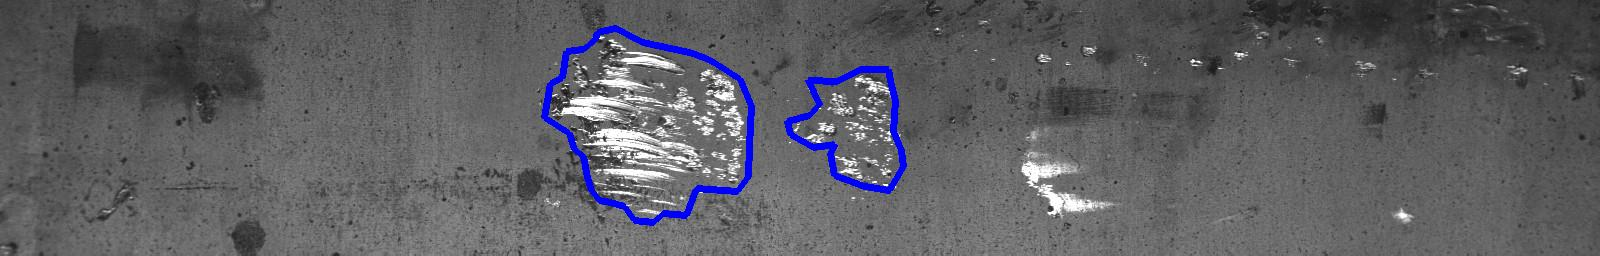
\includegraphics[width=\textwidth]{graphics/results/detector-result-class3-1}
	}
	\only<2-4> {
		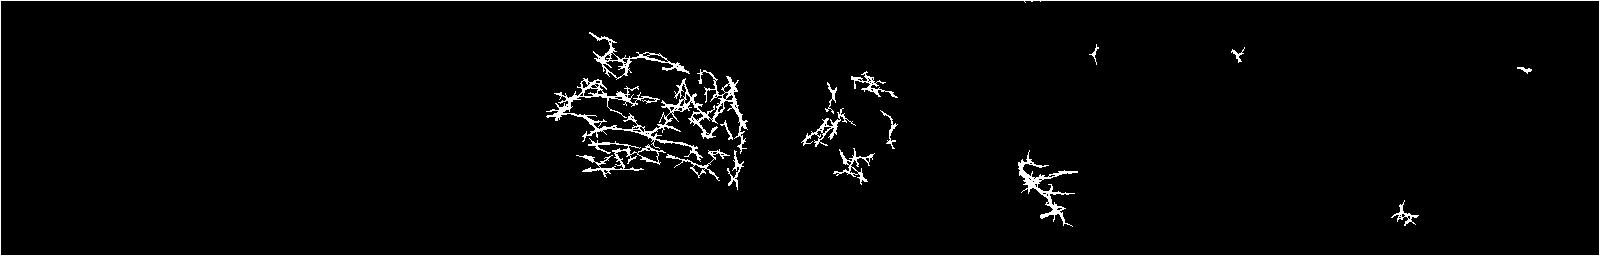
\includegraphics[width=\textwidth]{graphics/results/detector-result-class3-2}
	}
	\only<3-4> {
		
\includegraphics[width=\textwidth]{graphics/results/detector-result-class3-3}
	}
	\only<4> {
		
\includegraphics[width=\textwidth]{graphics/results/detector-result-class3-4}
	}
\end{frame}

\begin{frame}
\frametitle{Region proposals}
\framesubtitle{Example: Class No.4}
	\only<1-4> {
		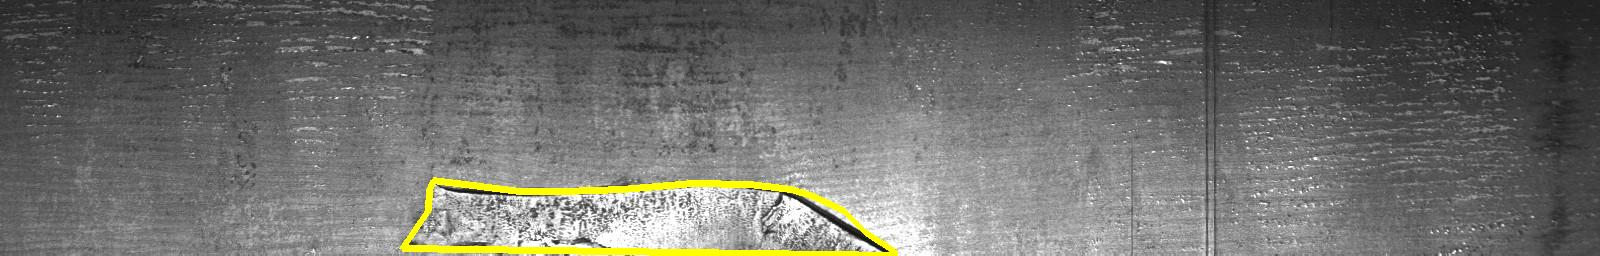
\includegraphics[width=\textwidth]{graphics/results/detector-result-class4-1}
	}
	\only<2-4> {
		
\includegraphics[width=\textwidth]{graphics/results/detector-result-class4-2}
	}
	\only<3-4> {
		
\includegraphics[width=\textwidth]{graphics/results/detector-result-class4-3}
	}
	\only<4> {
		
\includegraphics[width=\textwidth]{graphics/results/detector-result-class4-4}
	}
\end{frame}

\subsubsection{MC-CNN}
\begin{frame}{Multi Column CNN (MC-CNN)}
    \centering
    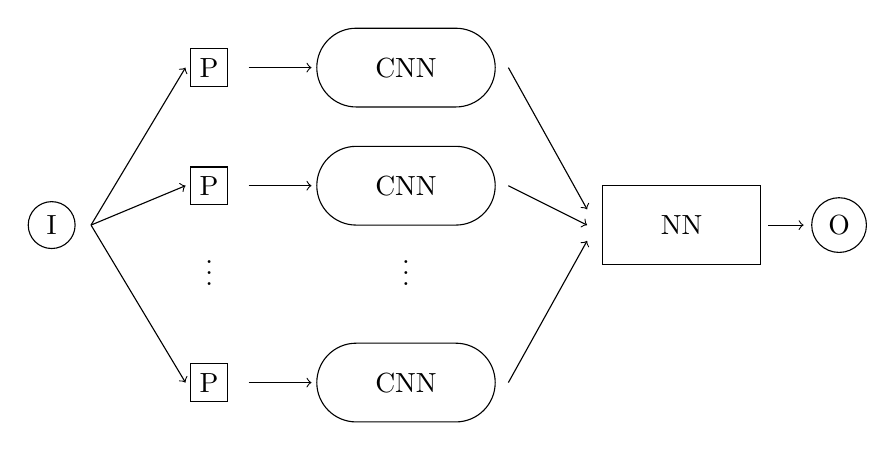
\begin{tikzpicture}
        % image
        \node[circle, draw] (input) at (0,0) {I};

        % preprocessed image
        \node[rectangle, draw] (p1) at ($(input) + (2,2)$) {P};
        \node[rectangle, draw] (p2) at ($(input) + (2,.5)$) {P};
        \node (p3) at ($(input) + (2,-.5)$) {\vdots};
        \node[rectangle, draw] (p4) at ($(input) + (2,-2)$) {P};

        % image to preprocessed image
        \draw[->] ($(input) + (0.5, 0)$) -- ($(p1) + (-0.3, 0)$);
        \draw[->] ($(input) + (0.5, 0)$) -- ($(p2) + (-0.3, 0)$);
        \draw[->] ($(input) + (0.5, 0)$) -- ($(p4) + (-0.3, 0)$);

        % cnn
        \node[rounded rectangle, draw, minimum width=2.5cm, minimum height=1cm] (cnn1) at ($(p1) + (2.5,0)$) {CNN};
        \node[rounded rectangle, draw, minimum width=2.5cm, minimum height=1cm] (cnn2) at ($(p2) + (2.5,0)$) {CNN};
        \node[minimum width=2.5cm, minimum height=1cm] (cnn3) at ($(p3) + (2.5,0)$) {\vdots};
        \node[rounded rectangle, draw, minimum width=2.5cm, minimum height=1cm] (cnn4) at ($(p4) + (2.5,0)$) {CNN};

        % preprocessed to cnn
        \draw[->] ($(p1) + (0.5, 0)$) -- ($(cnn1) + (-1.2, 0)$);
        \draw[->] ($(p2) + (0.5, 0)$) -- ($(cnn2) + (-1.2, 0)$);
        \draw[->] ($(p4) + (0.5, 0)$) -- ($(cnn4) + (-1.2, 0)$);

        % classifier
        \node[rectangle, draw, minimum width=2cm, minimum height=1cm] (classifier) at ($(cnn3) + (3.5,0.5)$) {NN};

        % cnn to classifier
        \draw[->] ($(cnn1) + (1.3, 0)$) -- ($(classifier) + (-1.2, .2)$);
        \draw[->] ($(cnn2) + (1.3, 0)$) -- ($(classifier) + (-1.2, 0)$);
        \draw[->] ($(cnn4) + (1.3, 0)$) -- ($(classifier) + (-1.2, -.2)$);

        % output
        \node[circle, draw] (output) at ($(classifier) + (2,0)$) {O};

        % classifier to output
        \draw[->] ($(classifier) + (1.1, 0)$) -- ($(output) + (-.45, 0)$);

    \end{tikzpicture}
\end{frame}

\begin{frame}{Multi Column CNN (MC-CNN)}
    \includegraphics[width=\textwidth]{graphics/architecture/mc-cnn-input}
    $$\Downarrow$$
    \centering
    \begin{tabular}{|c|c|c|c|c|}
        \hline
        Flawless area & Defect \#1 & Defect \#2 & Defect \#3 & Defect \#4\\\hline
        $1\%$ & $4\%$ & $6\%$ & \cellcolor{UniBlue}\textcolor{white}{$87\%$} & $2\%$ \\
        \hline
    \end{tabular}
\end{frame}

% \begin{frame}
%     \frametitle{Multi Column CNN (MC-CNN)}
%     \framesubtitle{Shape column}
%     \includegraphics[width=\textwidth]{graphics/architecture/mc-cnn-shape}
%     % \includegraphics[width=\textwidth]{graphics/architecture/mc-cnn-shape-architecture}
%     TODO confusion matrix + learning curve
% \end{frame}

% \begin{frame}
%     \frametitle{Multi Column CNN (MC-CNN)}
%     \framesubtitle{Local column}
%     \includegraphics[width=\textwidth]{graphics/architecture/mc-cnn-local}
%     % \includegraphics[width=\textwidth]{graphics/architecture/mc-cnn-shape-architecture}
%     TODO confusion matrix + learning curve
% \end{frame}

% \begin{frame}
%     \frametitle{Multi Column CNN (MC-CNN)}
%     \framesubtitle{Global column}
%     \includegraphics[width=\textwidth]{graphics/architecture/mc-cnn-global}
%     % \includegraphics[width=\textwidth]{graphics/architecture/mc-cnn-shape-architecture}
%     TODO confusion matrix + learning curve
% \end{frame}

\subsubsection{Output layer}
\begin{frame}{Output layer}
    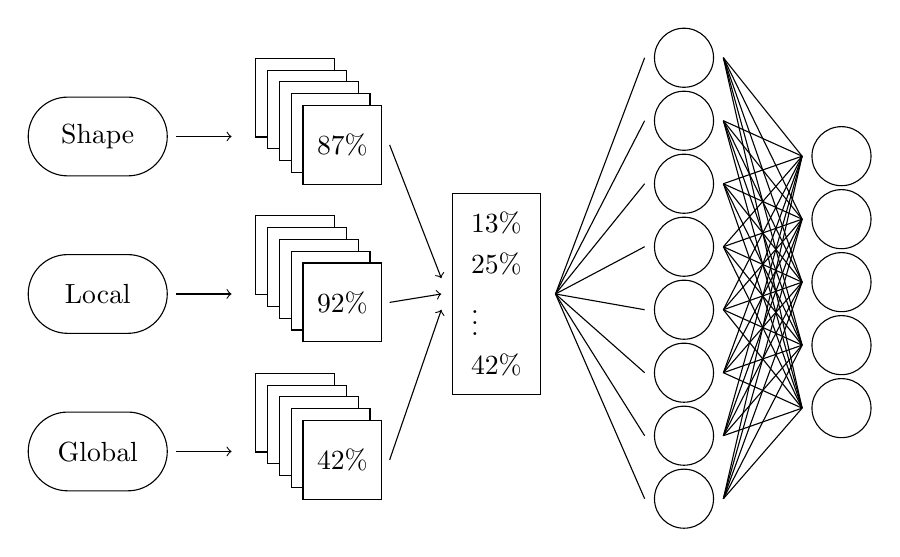
\begin{tikzpicture}

        % columns
        \node[rounded rectangle, draw, minimum width = 2cm, minimum height=1cm] (cnn1) at (0,2) {Shape};
        \node[rounded rectangle, draw, minimum width = 2cm, minimum height=1cm] (cnn2) at (0,0) {Local};
        \node[rounded rectangle, draw, minimum width = 2cm, minimum height=1cm] (cnn3) at (0,-2) {Global};

        % columns output
        \foreach \i in {0,...,4}
            \node[rectangle, draw, minimum width=1cm, minimum height=1cm, anchor=north west, fill=white] (output1 \i) at ($(cnn1) + (2+\i*0.15, 1-\i*.15) $) {$87\%$};

        \foreach \i in {0,...,4}
            \node[rectangle, draw, minimum width=1cm, minimum height=1cm, anchor=north west, fill=white] (output2 \i) at ($(cnn2) + (2+\i*0.15, 1-\i*.15) $) {$92\%$};

        \foreach \i in {0,...,4}
            \node[rectangle, draw, minimum width=1cm, minimum height=1cm, anchor=north west, fill=white] (output3 \i) at ($(cnn3) + (2+\i*0.15, 1-\i*.15) $) {$42\%$};

        % columns to output
        \draw[->] ($(cnn1) + (1, 0)$) -- ($(cnn1) + (1.7, 0)$);
        \draw[->] ($(cnn2) + (1, 0)$) -- ($(cnn2) + (1.7, 0)$);
        \draw[->] ($(cnn3) + (1, 0)$) -- ($(cnn3) + (1.7, 0)$);

        % fuse output
        \node [matrix, anchor=west, draw] (finalinput) at ($(cnn2) + (4.5,0)$)
        {
            \node {$13\%$};\\
            \node {$25\%$};\\
            \node {\vdots};\\
            \node {$42\%$};\\
        };

        % cnn output to flatten
        \draw[->] ($(output1 4) + (.6, 0)$) -- ($(finalinput) + (-.7,.2)$);
        \draw[->] ($(output2 4) + (.6, 0)$) -- ($(finalinput) + (-.7,0)$);
        \draw[->] ($(output3 4) + (.6, 0)$) -- ($(finalinput) + (-.7,-.2)$);

        % hidden layer
        \foreach \i in {0,...,7}
            \node[circle, draw, minimum width=.75cm, minimum height=.75cm, anchor=west] (h \i) at ($(finalinput) + (2, 3-\i*.8) $) {};
        \foreach \i in {0,...,7}
            \draw ($(finalinput) + (.75,0)$) -- ($(h \i) + (-.5,0)$);

        % output layer
        \foreach \i in {0,...,4}
            \node[circle, draw, minimum width=.75cm, minimum height=.75cm, anchor=west] (o \i) at ($(finalinput) + (4, 1.75-\i*.8) $) {};
        \foreach \i in {0,...,4}
            \foreach \j in {0,...,7}
                \draw ($(h \j) + (.5,0)$) -- ($(o \i) + (-.5,0)$);
        
        
    \end{tikzpicture}
    % FC NN + bayesopt params....
\end{frame}

\begin{frame}
    \frametitle{Multi Column CNN (MC-CNN)}
    \framesubtitle{Local column}
    \begin{columns}
        \column{.5\textwidth}
            Hello
%        \only<2> {
%            \column{.25}
%                % \includegraphics[height=\linewidth, angle=90, origin=c]{graphics/architecture/act_net}
%            \column{.25}
%                % \includegraphics[height=\linewidth, angle=90, origin=c]{graphics/architecture/act_net_hope}
%        }
    \end{columns}
\end{frame}


\subsection{Challenger}
\begin{frame}
    \frametitle{Challenger}
    \framesubtitle{Sliding window}
    \centering
    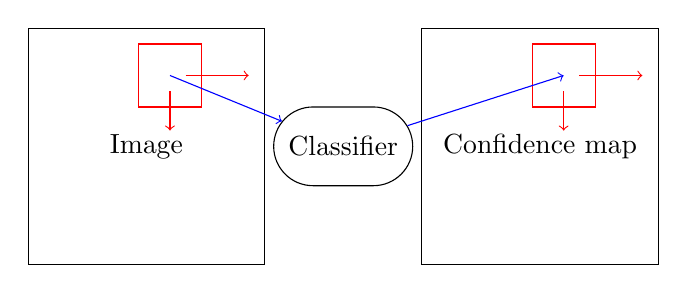
\begin{tikzpicture}
        % Image
        \node[rectangle, draw, minimum width=3cm, minimum height=3cm] (image) at (0,0) {Image};
        % Window
        \node[rectangle, draw=red, minimum width=.8cm, minimum height=.8cm] (window) at ($(image) + (.3,.9)$) {};
        % Sliding window
        \draw[->, draw=red] ($(window) + (.2,0)$) -- ($(window) + (1,0)$);
        \draw[->, draw=red] ($(window) + (0,-.2)$) -- ($(window) + (0,-.7)$);
        % Classifier
        \node[rounded rectangle, draw, minimum width=2cm, minimum height=1cm] (classifier) at ($(image) + (2.5,0)$) {Classifier};
        \draw[->,draw=blue] ($(window) + (0,0)$) -- (classifier);
        % Confidence map
        \node[rectangle,draw,minimum width=3cm, minimum height=3cm] (confidence map) at ($(classifier) + (2.5,0)$) {Confidence map};
        \node[rectangle, draw=red, minimum width=.8cm, minimum height=.8cm] (confidence map window) at ($(confidence map) + (.3,.9)$) {};
        \draw[->, draw=red] ($(confidence map window) + (.2,0)$) -- ($(confidence map window) + (1,0)$);
        \draw[->, draw=red] ($(confidence map window) + (0,-.2)$) -- ($(confidence map window) + (0,-.7)$);
        \draw[->,draw=blue] (classifier) -- ($(confidence map window)$);
    \end{tikzpicture}
\end{frame}

% \begin{frame}
%     \frametitle{Challenger}
%     \framesubtitle{Landmarks}
% \end{frame}
\section{Results}
    \begin{frame}{Results}
        \begin{center}
            \begin{tabular}{ |c|c|c|c|c|c|c| } 
             \hline
             Architecture & DCA [$\%$] & PCA [$\%$] & Overall Accuracy [$\%$]\\\hline
             Landmark & $90.24$ & $72.56$ & $80.94$\\ 
             Whatershed & $96.24$ & $82.56$ & $85.94$\\ 
             Proposed & $94.13$ & $93.16$ & $91.06$\\
             \hline
            \end{tabular}
            \vskip 1.5cm
            The project can be found in the \href{https://github.com/antonioterpin/wavelet_ml}{\texttt{GitHub repository}}
            \vskip 0.5cm
            \url{https://github.com/antonioterpin/wavelet_ml}
        \end{center}
    \end{frame}

% \begin{frame}[t,allowframebreaks]
% \frametitle{Bibliography}

% \nocite{*} % will display the non-cited publications as well. Useful for a publication list.

% \printbibliography

% \end{frame}

\end{document}